\documentclass{tufte-handout}

%\geometry{showframe}% for debugging purposes -- displays the margins

\usepackage{amsmath}

% Set up the images/graphics package
\usepackage{graphicx}
\setkeys{Gin}{width=\linewidth,totalheight=\textheight,keepaspectratio}
%\graphicspath{{graphics/}}

\title{Cloc drift and power sharing}
\author[Manel Velasco, Miguel Castilla]{Manel Velasco, Miguel Castilla}
%\date{ 19 January 2009}  % if the \date{} command is left out, the current date will be used
\date{dimarts, 19 de juliol de 2016}

% The following package makes prettier tables.  We're all about the bling!
\usepackage{booktabs}

% The units package provides nice, non-stacked fractions and better spacing
% for units.
\usepackage{units}

% The fancyvrb package lets us customize the formatting of verbatim
% environments.  We use a slightly smaller font.
\usepackage{fancyvrb}
\fvset{fontsize=\normalsize}

% Small sections of multiple columns
\usepackage{multicol}

% Provides paragraphs of dummy text
\usepackage{lipsum}

\usepackage[spanish]{babel}
\selectlanguage{spanish}
\usepackage[utf8]{inputenc}
   \setcounter{secnumdepth}{1} 

% These commands are used to pretty-print LaTeX commands
\newcommand{\doccmd}[1]{\texttt{\textbackslash#1}}% command name -- adds backslash automatically
\newcommand{\docopt}[1]{\ensuremath{\langle}\textrm{\textit{#1}}\ensuremath{\rangle}}% optional command argument
\newcommand{\docarg}[1]{\textrm{\textit{#1}}}% (required) command argument
\newenvironment{docspec}{\begin{quote}\noindent}{\end{quote}}% command specification environment
\newcommand{\docenv}[1]{\textsf{#1}}% environment name
\newcommand{\docpkg}[1]{\texttt{#1}}% package name
\newcommand{\doccls}[1]{\texttt{#1}}% document class name
\newcommand{\docclsopt}[1]{\texttt{#1}}% document class option name

\begin{document}

\maketitle% this prints the handout title, author, and date

\begin{abstract}
\noindent Este archivo sólo sirve para ordenar mi manera de pensar, no se puede esperar de é que sea serio ni concreto ni que se centre en una idea en particular ni que clarifique las ideas a nadie. 

El "drift" de los relojes de un sistema distribuido puede producir variaciones sensibles en los resultados finales de los puntos de equilibrio del sistema. Especialmente si el sistema tiene integradores. En este documento revisamos las ecuaciones para el lazo secundario del droop en una microred para intentar cuantificar sus efectos. 
\end{abstract}

%\printclassoptions

Antes de empezar debemos decir que nadie en la red posee un reloj perfecto, todos los generadores piensan que su reloj es el que funciona correctamente y ninguno de los generadores tiene constancia que el resto de generadores puedan tener un problema con sus relojes. Esto produce dos problemas fundamentales, por un lado cada uno de ellos generará una frecuencia de oscilación ligeramente diferente, pero el droop los forzará a que esta frecuencia sea exactamente la misma\sidenote{Nos referimos a físicamente la misma. Es decir, el droop fuerza a que todos los generadores funcionen a la misma frecuencia, aunque ellos consideren que sus frecuencias individualmente sean diferentes.} para todos ellos, pero, cada uno de ellos medirá\sidenote{No se mide nada, en realidad es una frecuencia que se genera. La confianza en el funcionamiento del reloj es tan grande que la generación de frecuencia funciona en lazo abierto. Nadie comprueba si la frecuencia generada y la consignada por la ecuación del droop son iguales, ni se cierra un lazo de control para forzar que sean iguales} una frecuencia de funcionamiento diferente, el resultado es que se produce un desbalanceo de carga. La segunda consecuencia es que el secundario verá la diferencia entre la frecuencia de consigna\sidenote{la frecuencia de consigna es $\omega_0$} y la frecuencia actual y generará un término para corregir el valor de funcionamiento. Nuevamente el droop hará que las frecuencia física de funcionamiento sea única para todos los generadores, y por lo general no coincidirá con ninguno de los valores que ellos creen que están generando. 


\section{Las ecuaciones de los relojes del sistema}
Hemos dicho que nadie posee un reloj perfecto, sin embargo es interesante disponer de un reloj perfecto para poder realizar un análisis del funcionamiento del sistema. Este reloj perfecto sólo existe desde un punto de vista analítico y sirve como marco de comparación entre los diferentes generadores. Podríamos escoger cualquiera de los generadores para considerar un marco de referencia global, pero esto le daría una importancia especial al generador que de hecho no tiene.

Para nosotros el tiempo global será la variable $t$, que nos sirve como marco de referencia para poder comparar los resultados que obtendremos. Nadie posee un reloj que sea capaz de medir de forma correcta a $t$, en general si medimos\sidenote{Medir el tiempo es un problema mayor, pero esto es un trabajo analítico y no hay problema en utilizar este lenguaje.} el tiempo con un generador $i$ y lo comparamos con el tiempo global obtenemos que 
\begin{align}
    \bar{t}_i(t)=f(t)
\end{align}
Una función del tiempo, que debería ser monótona creciente\sidenote{no permitimos viajes en el tiempo en este trabajo.}. Si el reloj del generador $i$ es suficientemente estable esta función es una recta
\begin{align}
    \bar{t}_i(t)=k_it+o_i
\end{align}
que tiene una pendiente $0<k_i<\infty$ y un offset respecto al reloj ideal. El offset es un elemento del que vamos a prescindir\sidenote{En los casos en los que sea importante lo marcaremos de forma explícita.}, puesto que estamos interesados en medir el paso del tiempo, no el tiempo en valor absoluto. Para ello podemos marcar un instante inicial de tiempo en el generador $\bar{T}_i(t=t_0)=k_it_0+o_i$ y consideraremos el tiempo en el generador como el intervalo de tiempo medido entre este punto inicial y cualquier otro instante de tiempo 
\begin{align}
    t_i=\bar{t}_i-\bar{T_i}=k_it+o_i-k_it_0-o_i=k_i\Delta t
\end{align}
Y de forma más laxa diremos que 
\begin{align}
t_i=k_it
\end{align}
para referirnos al paso del tiempo medido en un generador, aunque debe ser entendido como una relación entre intervalos de tiempos de dos relojes diferentes.

\section{Relación de frecuencias}

Dado un generador $i$, si éste genera una sinusoidal de  frecuencia $\omega$ con su reloj, ¿Cuál será la frecuencia vista desde el marco de referencia ideal?. Para verlo, expresamos las ecuaciones de la sinusoidal generada por el generador en términos del reloj ideal
\begin{align}
    sin(\omega t_i)=sin(\omega k_i t)=sin(\omega't)
\end{align}

Es decir, la frecuencia vista desde fuera será $\omega'=\omega k_i$, si el reloj del generador $i$ va más rápido esta frecuencia vista desde fuera será más alta de los esperado, si el reloj va mas lento, esta frecuencia será más lenta. Esto indica que hace falta distinguir el marco de referencia en el cual se generan las frecuencias, así si escribimos $\omega_i$ nos referimos a la frecuencia generada por el generador $i$ con su base de tiempo $t_i$. La ausencia de subíndice indica que la frecuencia se expresa en la base de tiempo ideal.

Esta notación nos permite establecer las relaciones entre los diferentes generadores, es decir, podemos ver como verá el generador $j$ una frecuencia generada por el generador $i$
\begin{align}
\omega=\omega_ik_i\\
\omega=\omega_jk_j\\
\omega_j=\omega_i\frac{k_i}{k_j}
\end{align}

Esta relación también establece que si dos generadores funcionan a la misma frecuencia\sidenote{Por ejemplo por efecto del droop} entonces\begin{align}
    \omega_ik_i=\omega_jk_j\label{fundamental1}
\end{align}
Sinedo $\omega_i$ y $\omega_j$ las frecuencias a las que ellos creen que están funcionando\sidenote{En la simulación con 2 generadores y drift ya hemos comprobado que esta relación existe}


\section{Desbalanceo del droop sin secundario debido al drift}
De la ecuacion \ref{fundamental1} se deduce rápidamente la relación de potencias un un sistema que utiliza el droop sin secundario
\begin{align}
\omega_ok_i-mP_ik_i=\omega_ok_j-mP_jk_j
\end{align}
Que nos lleva a 

\begin{align}
    P_i=P_j\frac{k_j}{k_i}+\omega_o\frac{(k_i-k_j)}{mk_i}\label{fundamental11}
\end{align}
 una relación lineal entre ellas y un offset, el offset tiene un efecto extraño, en situaciones de poca carga uno de los dos generadores se verá obligado a absorber carga en lugar de entregarla, lo que nos indica que en situaciones de poca carga hay que minimizar el número de generadores en la red. Otra interpretación sería que la diferencia en los relojes genera una carga virtual en la red, dado que no existe físicamente alguien la tiene que absorber la potencia generada.

 El resultado es que la potencia \textbf{no} puede ser la misma en todos los generadores debido a la diferencia entre los relojes de los generadores\sidenote{Se puede leer de muchas maneras diferentes, parece que cuantos más generadores hay peor es la situación}.Además el resultado dice que la diferencia de potencias depende de un offset que es inversamente proporcional a $m$, que es un elemento de diseño y de estabilidad del sistema, para $m$ muy pequeña las diferencias se acentúan notablemente, resultado que ya hemos visto en las simulaciones. Por otra parte, la ecuación \ref{fundamental11} abre la puerta a encontrar los valores de $k_i, k_j$ en un sistema, si medimos la diferencia de potencia entre ellos podemos tener una relación bastante buena de drift entre los relojes.

 Un aspecto a explotar de la ecuación es el hecho que el término de offset depende de la consigna $\omega_0$, a lo mejor se puede sacar partido a este hecho alterando los valores de consigna para intentar evaluar el comportamiento de los demás generadores y así reducir el desbalanceo. 
 


 \subsection{Resultados de simulación con 2 generadores}
 Si realizamos una simulación con dos generadores y comparamos los resultados obtenidos con los de la ecuación \ref{fundamental11} podremos comprobar si se cumple.

 Para esta simulación se ha utilizado el esquema que se muestra en la figura \ref{fig:modelo_droop_no_sec}, la carga variable se mantiene constante durante toda la simulación 
\begin{marginfigure}%
  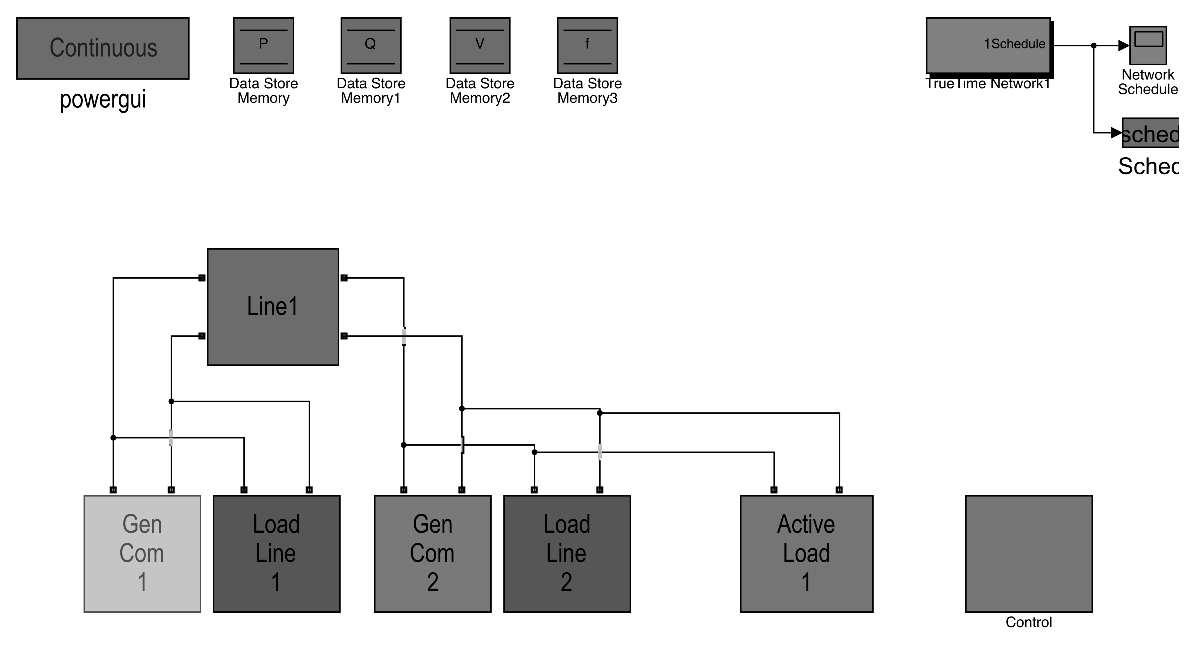
\includegraphics[width=\linewidth]{modelo_no_comm_no_sec}
  \caption{Modelo de la simulación}
  \label{fig:modelo_droop_no_sec}
\end{marginfigure}

 Para la simulación tenemos los siguientes datos:
 \begin{align}
     \begin{matrix}
         m=0.1\times10^{-6}\frac{\text{Rad}}{\text{J}} & k_1=1+50\times 10^{-6}\frac{s_1}{s}\\
         k_2=1\frac{s_2}{s} & w_0=50\text{Hz}  
     \end{matrix}
 \end{align}

\begin{marginfigure}%
  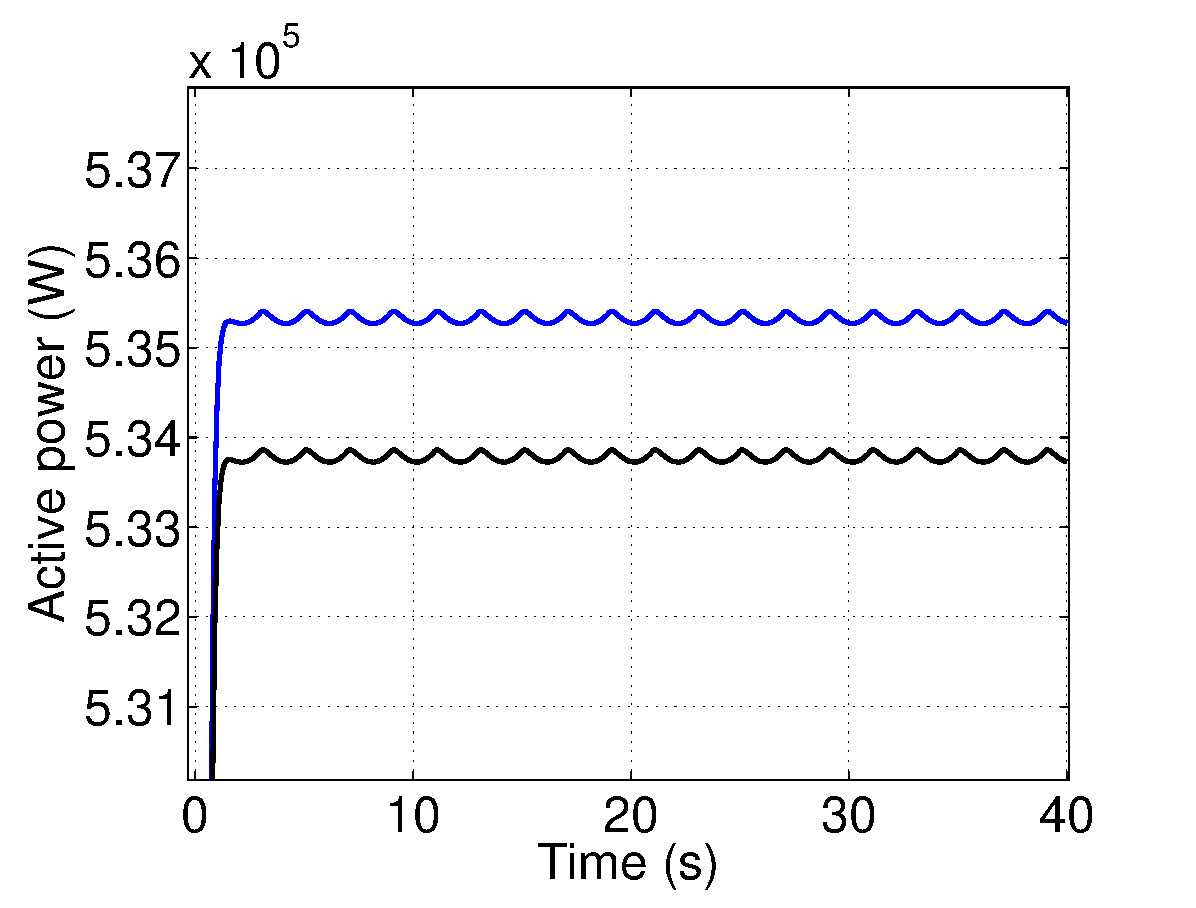
\includegraphics[width=\linewidth]{P_no_comm_no_sec}
  \caption{Detalle del valor de las potencias de dos generadores, sin comunicaciones, sin secundario.}
  \label{fig:p_droop_no_sec}
\end{marginfigure}
\begin{marginfigure}%
  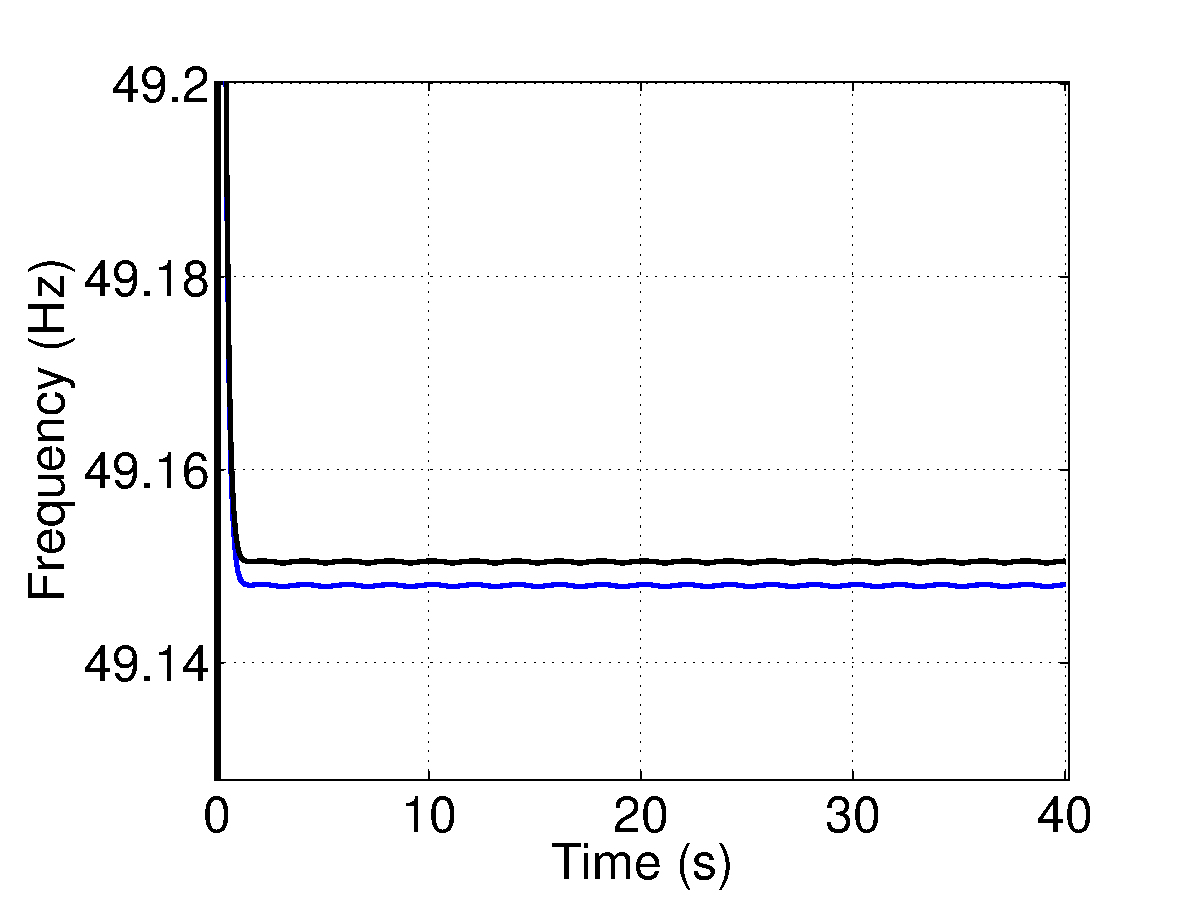
\includegraphics[width=\linewidth]{F_no_comm_no_sec}
  \caption{Detalle del valor de las frecuencias de dos generadores sin comunicaciones sin secundario. Medidas locales de frecuencia}
  \label{fig:f_droop_no_sec}
\end{marginfigure}
La figura \ref{fig:p_droop_no_sec} muestra los detalles del desbalanceo en la potencia tras la simulación y la figura \ref{fig:f_droop_no_sec} los detalles de la convergencia de las frecuencias. La medida de las frecuencias no coincide porque están expresadas en términos de los relojes locales, pero su valor físico es el mismo.
Las potencias medias obtenidas con estos datos son
\begin{align}
    P_1=5.353233533\times10^5 \text{Watt} &\, &  P_2=5.337793196\times10^5 \text{Watt}\\
    \omega_1=49.148006421 \text{Hz} &\, & \omega_2=49.150463827\text{Hz}
\end{align}
Aplicando la ecuación \ref{fundamental11} para calcular el valor de $P_1$ a partir del valor de $P_2$ obtenemos
\begin{align}
    P_1&=P_2\frac{k_2}{k_1}+\omega_o\frac{(k_1-k_2)}{mk_1}=\\
       &=5.337793196\times10^5\frac{1}{1.00005}+314.15\frac{(1.00005-1)}{0.1\times10^{-6}\times1.00005}=\\
       &=5.353233498340623\times10^5\,\text{Watt}
\end{align}
Este resultado coincide hasta el primer decimal con el resultado de la simulación.

\subsection{Resultados de la simulación con 4 generadores}
Para el caso de 4 generadores tomamos los siguientes valores

 \begin{align}
     \begin{matrix}
         m=0.1\times10^{-6}\frac{\text{Rad}}{\text{J}} & w_0=50\text{Hz}\\
         k_1=1+50\times 10^{-6}\frac{s_1}{s} & k_2=1\frac{s_2}{s}\\
         k_3=1+30\times 10^{-6} \frac{s_3}{s}& k_4=1-20\times10^{-6}\frac{s_4}{s} 
     \end{matrix}
 \end{align}
\begin{marginfigure}%
  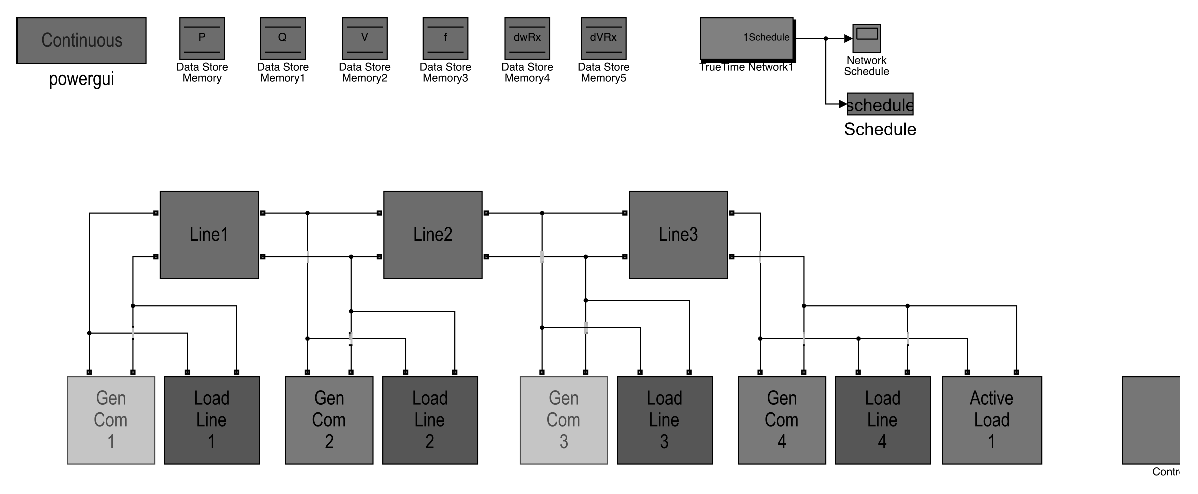
\includegraphics[width=\linewidth]{modelo_no_comm_no_sec_4_nod}
  \caption{Modelo de la simulación para 4 generadores sin comunicaciones y sin secundario}
  \label{fig:modelo_droop_no_sec_4}
\end{marginfigure}
El modelo de la simulación es el que se muestra en la figura \ref{fig:modelo_droop_no_sec_4}

Las gràficas de potencia y frecuencia para éste experimento se muestran en las figuras \ref{fig:p_droop_no_sec_4} y \ref{fig:f_droop_no_sec_4}

Los resultados de la simulación son
\begin{align}
    P_1=5.110704192\times10^5 \text{Watt} &\, &  P_2=5.095251956\times10^5 \text{Watt}\\
    P_3=5.101433256\times10^5  \text{Watt}& \, & P_4= 5.085979603\times10^5  \text{Watt}\\
    \omega_1=49.18660616 \text{Hz} &\, & \omega_2=49.18906546\text{Hz}\\
    \omega_3=49.188081681  \text{Hz}&\,& \omega_4=49.19054120  \text{Hz}
\end{align}
\begin{marginfigure}%
  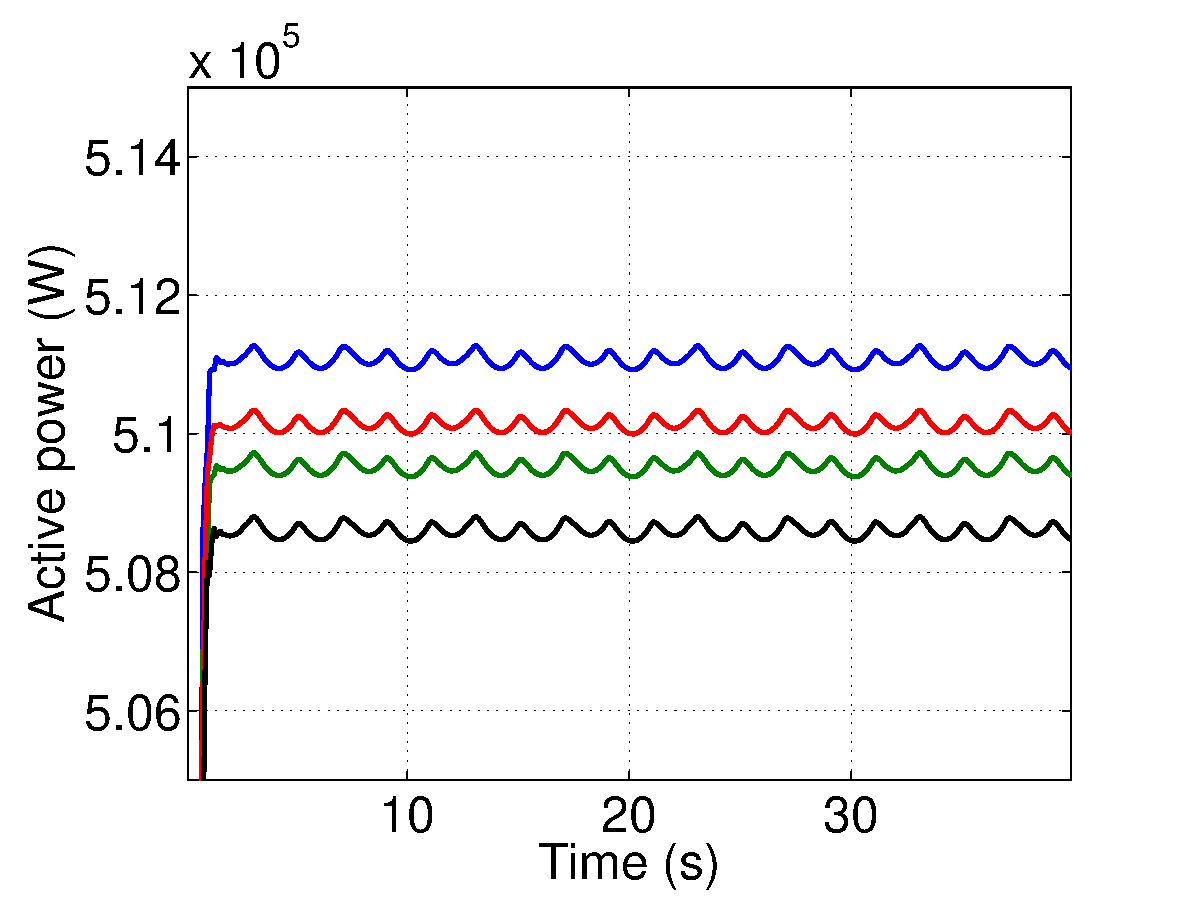
\includegraphics[width=\linewidth]{P_no_comm_no_sec_4}
  \caption{Detalle del valor de las potencias de cuatro generadores, sin comunicaciones, sin secundario.}
  \label{fig:p_droop_no_sec_4}
\end{marginfigure}
\begin{marginfigure}%
  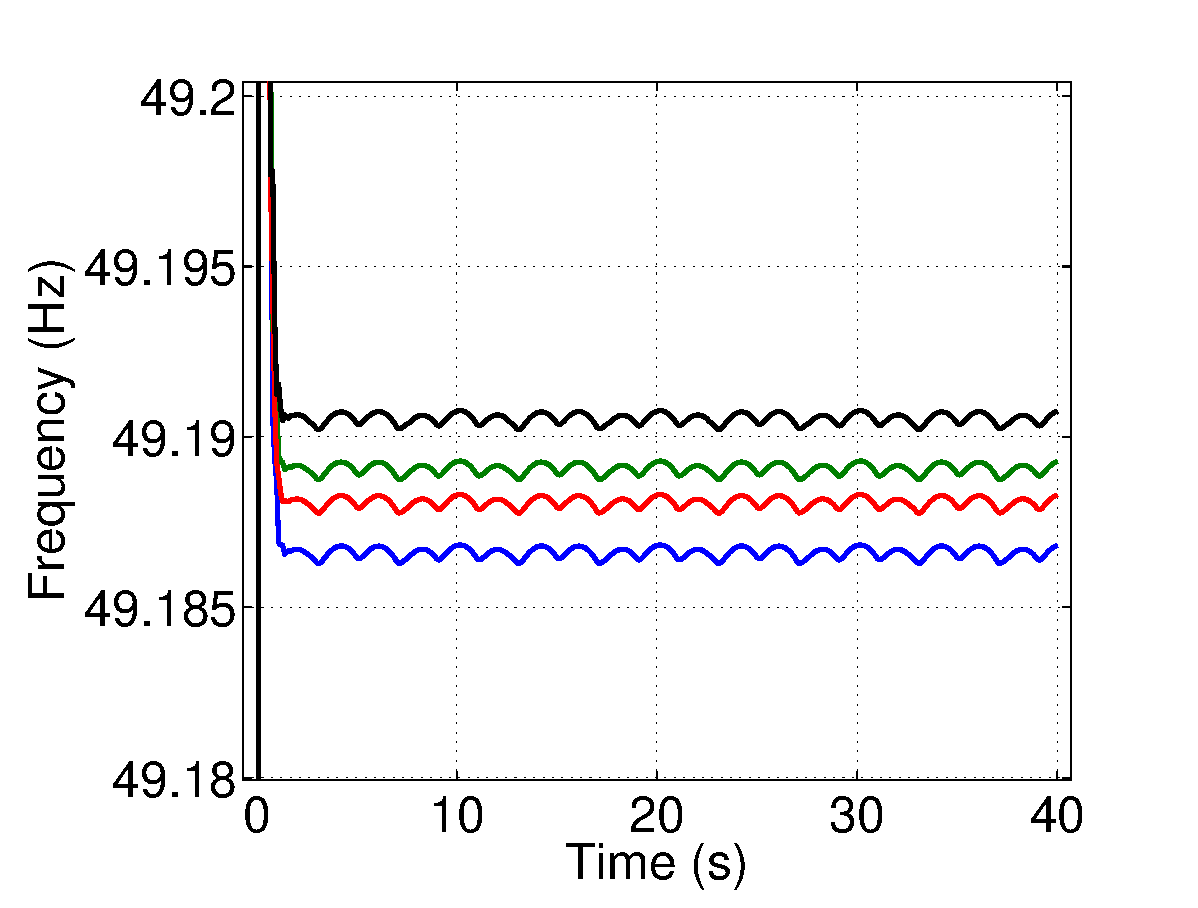
\includegraphics[width=\linewidth]{F_no_comm_no_sec_4}
  \caption{Detalle del valor de las frecuencias de cuatro generadores sin comunicaciones sin secundario. Medidas locales de frecuencia}
  \label{fig:f_droop_no_sec_4}
\end{marginfigure}
Para comprobar los resultados utilizamos la ecuación \ref{fundamental11} para calcular $P_1,P_2$ y $P_3$ a partir de $P_4$, lo que da como resultado

\begin{align}
    P_1=5.110704229\times10^5 \text{Watt} \\
    P_2=5.095251801\times10^5 \text{Watt}\\
    P_3=5.101432958\times10^5  \text{Watt}
\end{align}

Que coinciden con los datos de simulación hasta el primer decimal en algunos casos.

\section{Desbalanceo del droop con secundario debido al drift}
Para esta sección utilizaremos de nuevo la ecuación \ref{fundamental1}, es decir, pensamos que el sistema funciona con una frecuencia única, aunque desde el punto de vista de los generadores cada uno ve una frecuencia diferente. Este punto no está claro, sabemos que la potencia diverge, pero vemos que la frecuencia es única, el uso de la ecuación es un poco una inferencia inductivista, no está completamente justificado su uso. Sin embargo este punto puede ser trabajado con mayor detalle más adelante.

La ecuación individual de droop con secundario es
\begin{align}
    \omega_i=\omega_0-mP_i+K_I\int_0^{t_i}\omega_0-\omega_i\, dt_i
\end{align}

Pasado bastante tiempo, sabemos que la frecuencia se estabiliza, por lo tanto podemos reescribir la ecuación como
\begin{align}
    \omega_i=\omega_0-mP_i+K_I(\omega_0-\omega_i)t_i
\end{align}

Aislando
\begin{align}
    \omega_i=\omega_0-\frac{mP_i}{1+K_It_i}
\end{align}

Si usamos la ecuación \ref{fundamental1} obtenemos

\begin{align}
    \omega_0k_i-\frac{mP_i}{1+K_It_i}k_i=\omega_0k_j-\frac{mP_j}{1+K_It_j}k_j
\end{align}




\section{Figures and Tables}\label{sec:figures-and-tables}
Images and graphics play an integral role in Tufte's work.
In addition to the standard \docenv{figure} and \docenv{tabular} environments,
this style provides special figure and table environments for full-width
floats.

Full page--width figures and tables may be placed in \docenv{figure*} or
\docenv{table*} environments.  To place figures or tables in the margin,
use the \docenv{marginfigure} or \docenv{margintable} environments as follows
(see figure~\ref{fig:marginfig}):


The \docenv{marginfigure} and \docenv{margintable} environments accept an optional parameter \docopt{offset} that adjusts the vertical position of the figure or table.  See the ``\nameref{sec:sidenotes}'' section above for examples.  The specifications are:
\begin{docspec}
  \doccmd{begin\{marginfigure\}[\docopt{offset}]}\\
  \qquad\ldots\\
  \doccmd{end\{marginfigure\}}\\
  \mbox{}\\
  \doccmd{begin\{margintable\}[\docopt{offset}]}\\
  \qquad\ldots\\
  \doccmd{end\{margintable\}}\\
\end{docspec}

Figure~\ref{fig:fullfig} is an example of the \Verb|figure*|
environment and figure~\ref{fig:textfig} is an example of the normal
\Verb|figure| environment.

\begin{figure*}[h]
  \includegraphics[width=\linewidth]{sine.pdf}%
  \caption{This graph shows $y = \sin x$ from about $x = [-10, 10]$.
  \emph{Notice that this figure takes up the full page width.}}%
  \label{fig:fullfig}%
\end{figure*}

\begin{figure}
  \includegraphics{hilbertcurves.pdf}
%  \checkparity This is an \pageparity\ page.%
  \caption{Hilbert curves of various degrees $n$.
  \emph{Notice that this figure only takes up the main textblock width.}}
  \label{fig:textfig}
  %\zsavepos{pos:textfig}
  \setfloatalignment{b}
\end{figure}

Table~\ref{tab:normaltab} shows table created with the \docpkg{booktabs}
package.  Notice the lack of vertical rules---they serve only to clutter
the table's data.

\begin{table}[ht]
  \centering
%  \fontfamily{ppl}\selectfont
  \begin{tabular}{ll}
    \toprule
    Margin & Length \\
    \midrule
    Paper width & \unit[8\nicefrac{1}{2}]{inches} \\
    Paper height & \unit[11]{inches} \\
    Textblock width & \unit[6\nicefrac{1}{2}]{inches} \\
    Textblock/sidenote gutter & \unit[\nicefrac{3}{8}]{inches} \\
    Sidenote width & \unit[2]{inches} \\
    \bottomrule
  \end{tabular}
  \caption{Here are the dimensions of the various margins used in the Tufte-handout class.}
  \label{tab:normaltab}
  %\zsavepos{pos:normaltab}
\end{table}

\section{Full-width text blocks}

In addition to the new float types, there is a \docenv{fullwidth}
environment that stretches across the main text block and the sidenotes
area.

\begin{Verbatim}
\begin{fullwidth}
Lorem ipsum dolor sit amet...
\end{fullwidth}
\end{Verbatim}

\begin{fullwidth}
\small\itshape\lipsum[1]
\end{fullwidth}

\section{Typography}\label{sec:typography}

\subsection{Typefaces}\label{sec:typefaces}
If the Palatino, \textsf{Helvetica}, and \texttt{Bera Mono} typefaces are installed, this style
will use them automatically.  Otherwise, we'll fall back on the Computer Modern
typefaces.

\subsection{Letterspacing}\label{sec:letterspacing}
This document class includes two new commands and some improvements on
existing commands for letterspacing.

When setting strings of \allcaps{ALL CAPS} or \smallcaps{small caps}, the
letter\-spacing---that is, the spacing between the letters---should be
increased slightly.\cite{Bringhurst2005}  The \Verb|\allcaps| command has proper letterspacing for
strings of \allcaps{FULL CAPITAL LETTERS}, and the \Verb|\smallcaps| command
has letterspacing for \smallcaps{small capital letters}.  These commands
will also automatically convert the case of the text to upper- or
lowercase, respectively.

The \Verb|\textsc| command has also been redefined to include
letterspacing.  The case of the \Verb|\textsc| argument is left as is,
however.  This allows one to use both uppercase and lowercase letters:
\textsc{The Initial Letters Of The Words In This Sentence Are Capitalized.}



\section{Installation}\label{sec:installation}
To install the Tufte-\LaTeX\ classes, simply drop the
following files into the same directory as your \texttt{.tex}
file:
\begin{quote}
  \ttfamily
  tufte-common.def\\
  tufte-handout.cls\\
  tufte-book.cls
\end{quote}

% TODO add instructions for installing it globally



\section{More Documentation}\label{sec:more-doc}
For more documentation on the Tufte-\LaTeX{} document classes (including commands not
mentioned in this handout), please see the sample book.

\section{Support}\label{sec:support}

The website for the Tufte-\LaTeX\ packages is located at
\url{http://code.google.com/p/tufte-latex/}.  On our website, you'll find
links to our \smallcaps{svn} repository, mailing lists, bug tracker, and documentation.

%\bibliography{sample-handout}
%\bibliographystyle{plainnat}



\end{document}
